%
% This is the LaTeX template file for lecture notes for EE 382C/EE 361C.
%
% To familiarize yourself with this template, the body contains
% some examples of its use.  Look them over.  Then you can
% run LaTeX on this file.  After you have LaTeXed this file then
% you can look over the result either by printing it out with
% dvips or using xdvi.
%
% This template is based on the template for Prof. Sinclair's CS 270.

\documentclass[twoside]{article}
\usepackage{graphicx}
\usepackage{lipsum}
\usepackage[font=small,skip=0pt]{caption}
\usepackage{url}
\usepackage{makecell}
\usepackage{listings}
\usepackage{subfig}
\usepackage{algorithmicx}
\usepackage{algorithm}
\usepackage{algpseudocode}
\usepackage{amsmath}
\usepackage{amsfonts}
\usepackage{amssymb}
\usepackage{mathtools}
\usepackage{tikz,pgfplots}
\usepackage{caption}
\usepackage{graphics}
\setlength{\oddsidemargin}{0.25 in}
\setlength{\evensidemargin}{-0.25 in}
\setlength{\topmargin}{-0.6 in}
\setlength{\textwidth}{6.5 in}
\setlength{\textheight}{8.5 in}
\setlength{\headsep}{0.75 in}
\setlength{\parindent}{0 in}
\setlength{\parskip}{0.1 in}

%
% The following commands set up the lecnum (lecture number)
% counter and make various numbering schemes work relative
% to the lecture number.
%
\newcounter{lecnum}
\renewcommand{\thepage}{\thelecnum-\arabic{page}}
\renewcommand{\thesection}{\thelecnum.\arabic{section}}
\renewcommand{\theequation}{\thelecnum.\arabic{equation}}
\renewcommand{\thefigure}{\thelecnum.\arabic{figure}}
\renewcommand{\thetable}{\thelecnum.\arabic{table}}

%
% The following macro is used to generate the header.
%
\newcommand{\lecture}[4]{
   \pagestyle{myheadings}
   \thispagestyle{plain}
   \newpage
   \setcounter{lecnum}{#1}
   \setcounter{page}{1}
   \noindent
   \begin{center}
   \framebox{
      \vbox{\vspace{2mm}
    \hbox to 6.28in { {\bf EE 382V: Social Computing
                        \hfill Fall 2018} }
       \vspace{4mm}
       \hbox to 6.28in { {\Large \hfill Lecture #1: #2  \hfill} }
       \vspace{2mm}
       \hbox to 6.28in { {\it Lecturer: #3 \hfill Scribe: #4} }
      \vspace{2mm}}
   }
   \end{center}
   \markboth{Lecture #1: #2}{Lecture #1: #2}
   %{\bf Disclaimer}: {\it These notes have not been subjected to the
   %usual scrutiny reserved for formal publications.  They may be distributed
   %outside this class only with the permission of the Instructor.}
   \vspace*{4mm}
}

%
% Convention for citations is authors' initials followed by the year.
% For example, to cite a paper by Leighton and Maggs you would type
% \cite{LM89}, and to cite a paper by Strassen you would type \cite{S69}.
% (To avoid bibliography problems, for now we redefine the \cite command.)
% Also commands that create a suitable format for the reference list.
\renewcommand{\cite}[1]{[#1]}
\def\beginrefs{\begin{list}%
        {[\arabic{equation}]}{\usecounter{equation}
         \setlength{\leftmargin}{2.0truecm}\setlength{\labelsep}{0.4truecm}%
         \setlength{\labelwidth}{1.6truecm}}}
\def\endrefs{\end{list}}
\def\bibentry#1{\item[\hbox{[#1]}]}

%Use this command for a figure; it puts a figure in wherever you want it.
%usage: \fig{NUMBER}{SPACE-IN-INCHES}{CAPTION}
\newcommand{\fig}[3]{
			\vspace{#2}
			\begin{center}
			Figure \thelecnum.#1:~#3
			\end{center}
	}
% Use these for theorems, lemmas, proofs, etc.
\newtheorem{theorem}{Theorem}[lecnum]
\newtheorem{lemma}[theorem]{Lemma}
\newtheorem{proposition}[theorem]{Proposition}
\newtheorem{claim}[theorem]{Claim}
\newtheorem{corollary}[theorem]{Corollary}
\newtheorem{definition}[theorem]{Definition}
\newenvironment{proof}{{\bf Proof:}}{\hfill\rule{2mm}{2mm}}

% **** IF YOU WANT TO DEFINE ADDITIONAL MACROS FOR YOURSELF, PUT THEM HERE:

\begin{document}
%FILL IN THE RIGHT INFO.
%\lecture{**LECTURE-NUMBER**}{**DATE**}{**LECTURER**}{**SCRIBE**}
\lecture{8}{November 10}{Vijay Garg}{Shiyang Cheng}
%\footnotetext{These notes are partially based on those of Nigel Mansell.}

% **** YOUR NOTES GO HERE:

% Some general latex examples and examples making use of the
% macros follow.  
%**** IN GENERAL, BE BRIEF. LONG SCRIBE NOTES, NO MATTER HOW WELL WRITTEN,
%**** ARE NEVER READ BY ANYBODY.
\section{Ceaser Cipher}
In cryptography, {\em Caeser Cipher} is one of the simplest encryption techniques.
It exploit substitution cipher in which each letter in the plaintext is replaced
by a letter some fixed number of postions down the alphabet.

For example:

Cipher:
$HPPE$ $NPSOJOH$

Plain:
$good$ $morning$

In which, $H$ maps to $g$, and so on.

\section{RSA - Asymmetric cryptography}
RSA stands for Rivest-Shamir-Adleman. 

\subsection{History}
Cryptanalysis of the Enigma ciphering system enabled the western Allies in World War II to read substantial amounts of Morse-coded radio communications of the Axis powers that had been enciphered using Enigma machines. This yielded military intelligence which, along with that from other decrypted Axis radio and teleprinter transmissions, was given the codename Ultra. This was considered by western Supreme Allied Commander Dwight D. Eisenhower to have been "decisive" to the Allied victory.

The Enigma machines were a family of portable cipher machines with rotor scramblers. Good operating procedures, properly enforced, would have made the plugboard Enigma machine unbreakable. However, most of the German military forces, secret services and civilian agencies that used Enigma employed poor operating procedures, and it was these poor procedures that allowed the Enigma machines to be reverse-engineered and the ciphers to be read.

The German plugboard-equipped Enigma became Nazi Germany's principal crypto-system. It was broken by the Polish General Staff's Cipher Bureau in December 1932, with the aid of French-supplied intelligence material obtained from a German spy. A month before the outbreak of World War II, at a conference held near Warsaw, the Polish Cipher Bureau shared its Enigma-breaking techniques and technology with the French and British. During the German invasion of Poland, core Polish Cipher Bureau personnel were evacuated, via Romania, to France where they established the PC Bruno signals intelligence station with French facilities support. Successful cooperation among the Poles, the French, and the British at Bletchley Park continued until June 1940, when France surrendered to the Germans.

From this beginning, the British Government Code and Cypher School (GC\&CS) at Bletchley Park built up an extensive cryptanalytic capability. Initially, the decryption was mainly of Luftwaffe (German air force) and a few Heer (German army) messages, as the Kriegsmarine (German navy) employed much more secure procedures for using Enigma. Alan Turing, a Cambridge University mathematician and logician, provided much of the original thinking that led to the design of the cryptanalytical bombe machines that were instrumental in eventually breaking the naval Enigma. However, the Kriegsmarine introduced an Enigma version with a fourth rotor for its U-boats, resulting in a prolonged period when these messages could not be decrypted. With the capture of relevant cipher keys and the use of much faster US Navy bombes, regular, rapid reading of U-boat messages resumed\cite{WikiEnigma}.


In 1970, \textit{James H. Ellis}, a British cryptographer at the UK Government 
Communications Headquarters (GCHQ), conceived of the possibility of 
"non-secret encryption", (now called public key cryptography), but could 
see no way to implement it. In 1973, his colleague \textit{Clifford Cocks} 
implemented what has become known as the RSA encryption algorithm, 
giving a practical method of "non-secret encryption", and in 1974, 
another GCHQ mathematician and cryptographer, \textit{Malcolm J. Williamson}, 
developed what is now known as \textit{{Diffie-Hellman}} key exchange\cite{WikiRSA}.

\subsection{RSA Use Case}
There are three individuals: \textit{Alice}, \textit{Bob}, \textit{Eve}.  
\textit{Alice} want to communicate with \textit{Bob} as figure-\ref{p1}.
\textit{Eve} is a passive attacker, who intercepts all the message between \textit{Alice}
and \textit{Bob}. \textit{Eve} also could send message to each other pretend to be one of them.
\textit{Alice} and \textit{Bob} want to keep the message secrecy and authentication
at the same time.

\begin{figure}[ht!]
\centering
    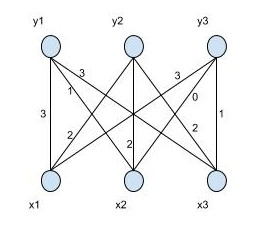
\includegraphics[width=50mm]{figure1}
\caption{RSA Use Case\label{p1}}
\end{figure}


Solution:
Let's define:

$e_A$: \textit{Alice}'s public key

$d_A$: \textit{Alice}'s private key

$e_B$: \textit{Bob}'s public key

$d_B$: \textit{Bob}'s private key

$E$: encryption function

$D$: decryption function

Assume that \textit{Alice} gets \textit{Bob}'s public key $e_A$,
and \textit{Bob} gets \textit{Alice}'s public key. Nobody shares private key to anyone.

\textit{Alice} want to send message $M$. She applies the encryption function to $M$,
using encryption function $E$ with \textit{Bob}'s public key $e_B$
as $E(M, e_B)$. Then encrypt the encrypted message again using her own private key
$d_A$, which is $E(E(M, e_B), d_A)$.

\textit{Bob} could use \textit{Alice}'s public key $e_A$ to decrypt the message into
$E(M, e_B)$. If and only if the message comes from \textit{Alice}, \textit{Bob} could
get the message $E(M, e_B)$, and decrypt the message again using his own private key
$d_B$ into message $M$.

In this way, \textit{Bob} use \textit{Alice}'s public key $e_A$ to authenticate 
\textit{Alice}. And use his own private $d_B$ to decrypt the message which 
provide the secrecy at the same time.

This procedure exploit the property that only $E(M, e)$, $D(E(M, e), d)$ is easy. 
And the other way $E(M, d)$, $D(E(M, d), e)$ are easy.

\subsection{RSA Algorithms}

\subsubsection{Generate Key Pairs}

\begin{algorithm}[H]
    \caption{generateKeyPair()}
\begin{algorithmic}

    \State 1. Take two big prime numbers $p$ and $q$, let $n=p^q$
    \\
    \State 2. Compute \textit{Euler}'s totient function $\Phi(n)=(p - 1)\ast(q - 1)$
    \\
    \State 3. Choose any number $e$ that relatively prime to $\Phi(n)$, which means
    $gcd(e, \Phi(n)) = 1$
    \\
    \State 4. Find $d$ such that $d\ast e = 1\; mod\; \Phi(n)$
    \\
    \State 5. throw away $p$, $q$, $\Phi(n)$
    \\
    \State 6. return $(n, e)$ as public key, $(n, d)$ as private key
\end{algorithmic}
    \label{keyPair}
\end{algorithm}
This section gives the algorithms is meant to generate key pair which is $(e, d) as algorithm-$\ref{keyPair}.
The function to encrypt message $M$ as $C$:

$C = M^e\; mod\; n$

The function to decrypt encrypted message $C$ back to $M$:

$M = C^d\; mod\; n$

\subsubsection{Modulo Properties}

\textit{Modulo} operation finds the remainder after division of one number by antoher,
which represent as $mod$.

\textit{Modulo} operation has properties:

1. $(a\, +\, b)\; mod\; n = ((a\; mod\; n) + (b\; mod\; n))$

2. $(a\, \ast\, b)\; mod\; n = ((a\; mod\; n) \ast\, (b\; mod\; n))$


\clearpage
\section*{References}
\beginrefs
\bibentry{WikiRSA}{\sc wikipedia},
Public-key cryptography
{\it wikipedia.org} (2018),

\bibentry{WikiEnigma}{\sc wikipedia},
Cryptanalysis of the Enigma
{\it wikipedia.org} (2018),

\endrefs


\end{document}





